\documentclass[conference]{IEEEtran}

\usepackage{cite}
\usepackage{amsmath,amssymb,amsfonts}
\usepackage{algorithmic}
\usepackage{graphicx}
\usepackage{textcomp}
\usepackage{xcolor}
\usepackage{hyperref}
\usepackage{multirow}
\usepackage{graphicx}
\usepackage{subcaption}
\def\BibTeX{{\rm B\kern-.05em{\sc i\kern-.025em b}\kern-.08em
    T\kern-.1667em\lower.7ex\hbox{E}\kern-.125emX}}

\hypersetup{
	colorlinks=true,
	linkcolor=black,
	filecolor=black,      
	urlcolor=black,
	citecolor=black
}
\begin{document}

\title{Characterizing High-Risk Environmental Signatures: An Unsupervised Approach to Predicting Traffic Accident Probability}

\author{\IEEEauthorblockN{Gabriel Guillen}
	\IEEEauthorblockA{\textit{dept. of Statistics \& Data Science} \\
		\textit{University of Central Florida}\\
		Orlando, United States of America \\
		ga013701@ucf.edu}}

\maketitle
\renewcommand{\abstractname}{Summary}
\begin{abstract}
This analysis maps the ``Perfect Storm" of Florida road safety by identifying the precise moments when environmental hazards and infrastructure vulnerabilities converge into car accident events. Utilizing an unsupervised learning framework—including PCA, K-Means, Gaussian Mixture Models, and Spectral Clustering—the study moves from broad trends to isolate three distinct dimensions of danger: macro-risk profiles, nuanced visibility triggers, and the ``Vulnerable Junctions" where structural gaps are most critical. Rather than offering design suggestions, these clusters define the specific situational signatures and non-linear interactions that cause a road environment to transition from manageable to high-risk. The result is a data-driven map of the specific driving windows and atmospheric thresholds that maximize crash probability across the state.
\end{abstract}

\section{\textbf{Introduction}}
Traffic safety is an emergent property, not a solo act. Factors like weather or visibility rarely cause crashes in isolation; instead, accidents spring from the complex, non-linear friction between drivers and their surroundings.\\
\indent This report seeks to move beyond traditional univariate analysis by characterizing the ``Perfect Storm": \textbf{a high-risk environmental signature where specific temporal, environmental, and situational factors converge to maximize crash probability.}\\
\indent The target of this analysis is to identify these latent, multi-dimensional patterns within a Florida-specific dataset of 881,605 traffic records. By applying an unsupervised learning framework—utilizing \textbf{Principal Component Analysis (PCA)} for dimensionality reduction followed by \textbf{K-Means}, \textbf{Gaussian Mixture Models (GMM)}, and \textbf{Spectral Clustering}—this study aims to pinpoint the exact intersections of visibility impairment, atmospheric conditions, and infrastructure vulnerability that define the most hazardous road environments in the state.\\
\indent Rather than general trends, this analysis isolates the "Perfect Storm" signatures—the precise moments where environmental hazards and design failures align. These profiles map the transition from manageable to high-risk, identifying the situational triggers that define Florida’s most dangerous driving windows.

\subsection{\textbf{Dataset Structure}}
\indent Derived from \cite{moosavi2019countrywide} and \cite{moosavi2019accident}, the dataset was procured via streaming APIs from the US Department of Transportation and law enforcement agencies. For this analysis, the data was narrowed to 881,605 Florida-specific observations.\\
\indent The structure incorporates 46 multidimensional features—including numeric environmental metrics (e.g., \texttt{Temperature(F)}, \texttt{Visibility(mi)}), categorical weather descriptors, and boolean road attributes (e.g., \texttt{Junction}, \texttt{Traffic\_Signal})—providing the necessary framework for unsupervised cluster analysis.

\vspace{2mm}

\section{\textbf{Methods}}

\subsection{\textbf{Data Preprocessing}}

To prevent feature redundancy and correlation ``bleeding'', the dataset was trimmed from 46 to 28 variables by removing geographic and descriptive identifiers. Missing data was handled via hybrid imputation: numeric values were filled using the median (44,050 rows) and categorical gaps using the mode (19,199 rows).

\subsubsection*{\textbf{Sensitivity Analysis}} 

\begin{figure}[htbp]
	\centerline{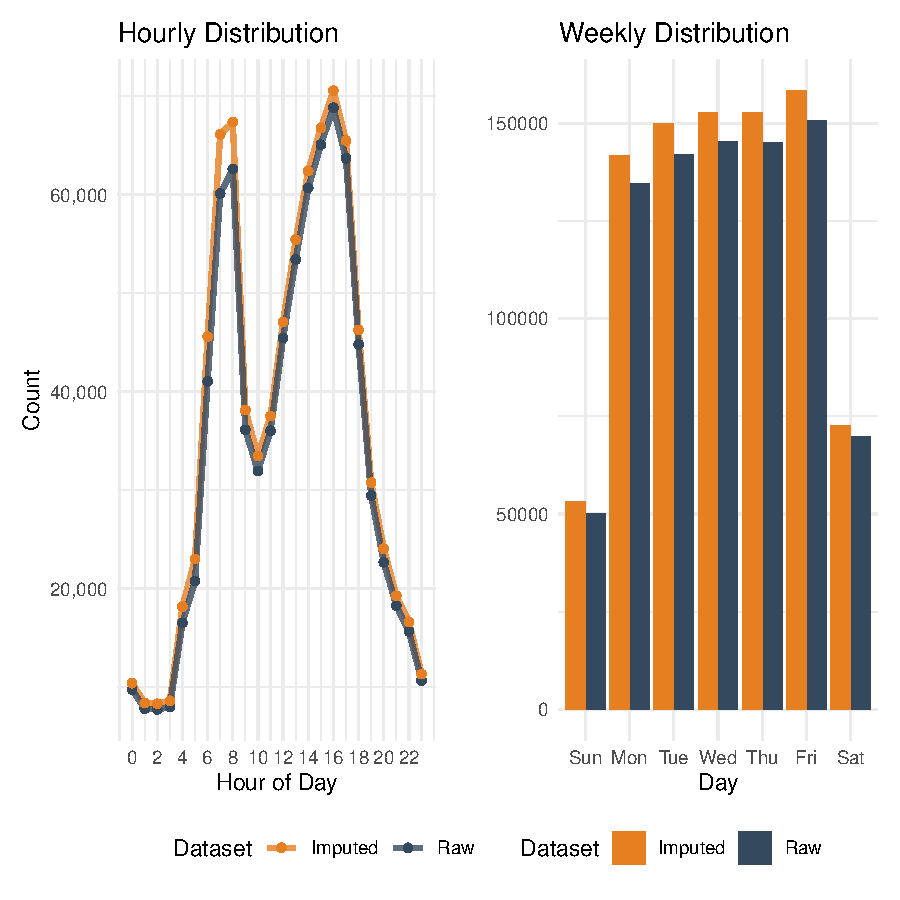
\includegraphics[scale=0.4]{temporal_analysis.pdf}}
	\caption{Time Features with Imputation}
	\label{temporal_analysis}
\end{figure}

\indent This process yielded a 5\% unique row-level manipulation rate, retaining 881,605 records compared to the 837,555 that would have remained under listwise deletion.

 
The 5\% imputation rate proved statistically non-significant, as variable distributions remained stable. The mean shift in temporal data was a negligible $-0.1342\%$ (displayed example in Figure \ref{temporal_analysis}). 

\begin{figure}[htbp]
	\centerline{
\includegraphics[scale=0.35]{categorical_sensitivity.pdf}}
	\caption{Categorical Sensitivity}
	\label{categorical_sensitivity}
\end{figure} 

While categorical proportions shifted by a maximum of only $\sim$0.04. This confirms that mode-based imputation preserved the underlying frequency of environmental conditions (Figure \ref{categorical_sensitivity}).

\subsubsection*{\textbf{Normalization}}
\indent Following feature engineering of temporal variables and the conversion of logical indicators into binary format, the analysis performed a zero-variance check to drop columns providing no discriminative power.\\
\indent The remaining features underwent \textbf{Z-score Normalization} \cite{ISLR2} (zero mean, unit variance) to ensure feature magnitude did not bias subsequent dimensionality reduction or clustering algorithms.

\vspace{2mm}

\subsection{\textbf{Exploratory Data Analysis (EDA)}}
With the dataset stabilized and standardized, the exploratory analysis focused on uncovering the underlying environmental and temporal patterns that characterize Florida's traffic risk.

\subsubsection*{\textbf{Temporal and Distributional Trends}} As shown in Figure \ref{temporal_analysis}, temporal data revealed a ``double-peak'' profile corresponding to morning (7:00--8:00 AM) and evening (3:00--5:00 PM) commutes. Incident volume peaked on Fridays (158,372), suggesting that high-density commuter cycles, rather than recreational travel, are the primary drivers of accidents frequency. 

\begin{figure}[htbp]
	\centerline{
\includegraphics[scale=0.40]{categorical_distribution_weather.pdf}}
	\caption{Weather Patterns Distribution}
	\label{categorical_distribution_weather}
\end{figure} 

\textbf{Weather:} Analysis of weather signatures, shown in Figure \ref{categorical_distribution_weather}, reveals a counterintuitive distribution: conditions typically associated with high risk—such as Heavy Rain or Fog—appear lower in the accident frequency distribution than expected. 

\textbf{Severity:} Where the severity of most accidents are mostly in Level 2 and 3, with low-impact and high-impact being in the minority of the accident's distribution, shown in Figure \ref{severity_detailed}.

\begin{figure}[htbp]
	\centerline{
\includegraphics[scale=0.35]{severity_detailed.pdf}}
	\caption{Severity Level Distribution}
	\label{severity_detailed}
\end{figure} 

\begin{figure}[htbp]
	\centerline{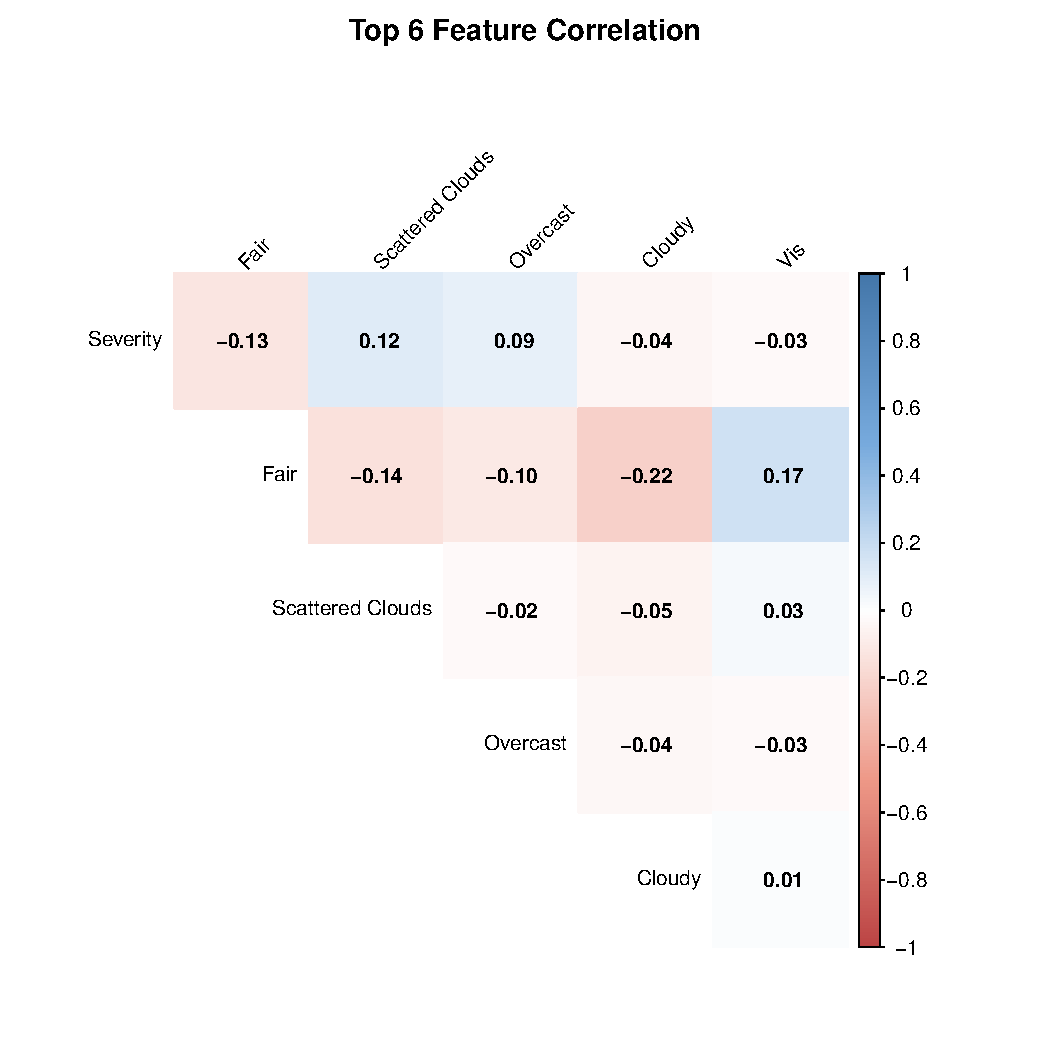
\includegraphics[scale=0.50]{Linear_Correlation.pdf}}
	\caption{Influences on Accidents Severity}
	\label{Linear_Correlation}
\end{figure} 

\textbf{Synergistic Risk Model:} While visibility or fair weather are intuitive drivers of accident severity, the data reveals only negligible linear correlations, specifically $r = -0.03$ and $r = -0.13$, respectively in Figure \ref{Linear_Correlation}.\\
\indent This suggests that severity is an emergent property of non-linear environmental interactions rather than individual factors. \\
\indent To uncover the latent patterns governing high-severity events obscured within the 28-variable feature space, we turn to \textbf{Dimensionality Reduction}.

\vspace{2mm}

\subsection{\textbf{Dimension Reduction}}

To address the high-dimensionality of the 28-variable feature space, two complementary reduction techniques were evaluated to identify the latent structures driving incident probability.

\begin{itemize}
	\item \textbf{Principal Component Analysis (PCA) \cite{Pearson1901}:} A linear method that transforms correlated variables into a set of linearly uncorrelated components. It is used here to capture the maximum global variance of the environmental data.
	\item \textbf{Uniform Manifold Approximation and Projection (UMAP) \cite{McInnes2018}:} A non-linear dimensionality reduction technique that preserves local topological structures. It serves as a diagnostic tool to determine if the ``Perfect Storm'' signatures are governed by complex, non-linear manifolds.
\end{itemize}

\subsubsection*{\textbf{Evaluation and Feature Selection}}
The selection of optimal features for subsequent clustering was guided by the following empirical observations:
\begin{figure}[htbp]
	\centerline{
\includegraphics[scale=0.50]{PCA_Combined_Scree_Plot.pdf}}
	\caption{PCA Scree Plot}
	\label{PCA_Combined_Scree_Plot}
\end{figure} 
\begin{enumerate}
	\item \textbf{Linear Variance Elbow:} The PCA Scree Plot (Figure \ref{PCA_Combined_Scree_Plot}) was used to determine the optimal number of Principal Components. The plot exhibits a distinct ``elbow'' where the last dramatic drop in explained variance occurs at the eighth component. Consequently, $PC_1$ through $PC_8$ were identified as capturing the essential linear signals of the dataset.
	
	\item \textbf{Weak Non-Linearity:} The UMAP Global Density Map (Figure \ref{UMAP_Density_Map}) displays a largely homogenous, circular distribution of 881,605 observations. The absence of distinct clusters, filaments, or separated manifolds in this global projection indicates that non-linear relationships between the features are relatively weak or lack sufficient local structure to justify non-linear clustering.
\end{enumerate}
\begin{figure}[htbp]
	\centerline{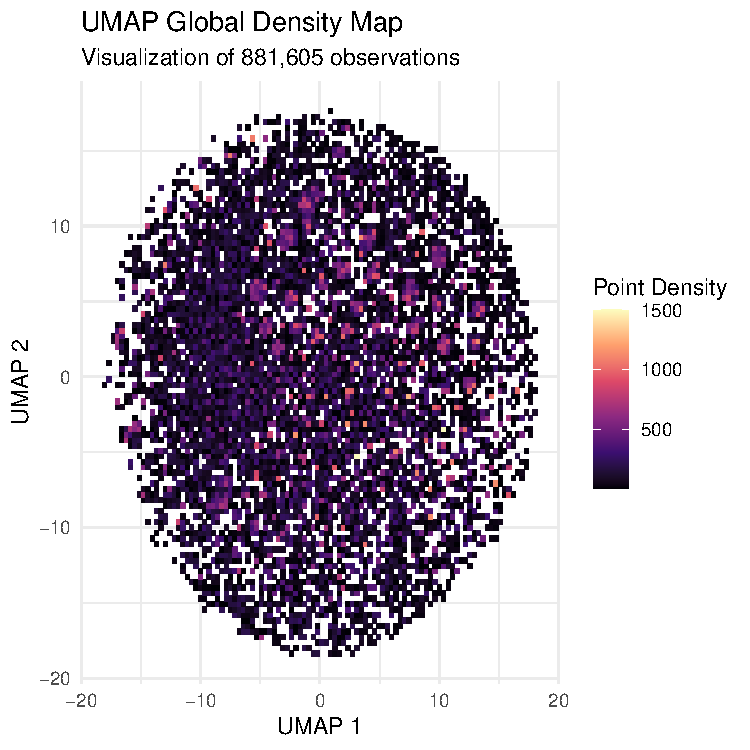
\includegraphics[scale=0.50]{UMAP_Density_Map.pdf}}
	\caption{UMAP Density Map}
	\label{UMAP_Density_Map}
\end{figure} 

Because the \textbf{UMAP} projection suggests that non-linear manifold structures are not a dominant feature of this dataset, the first eight Principal Components ($PC_1$--$PC_8$) will be utilized as the primary inputs for the subsequent clustering models.\\
\indent This ensures the clustering focuses on the core environmental drivers without unnecessary complexity.

\vspace{2mm}

\subsection{\textbf{Clustering Framework}}
To identify the distinct environmental signatures associated with accident probability, the first eight Principal Components ($PC_1$--$PC_8$) are utilized as the input feature space. This ensures that the clustering algorithms operate on the most significant variance in the dataset while mitigating the impact of collinearity among raw environmental variables. Three distinct models are evaluated to identify the ``Perfect Storm" clusters:

\begin{itemize}
	\item \textbf{K-Means Clustering \cite{MacQueen1967}:} A centroid-based algorithm that partitions the PC-space into $k$ clusters by minimizing the squared Euclidean distance between data points and their respective cluster centers. This model provides a clear, geometric partitioning of environmental risk profiles.
	
	\item \textbf{Gaussian Mixture Models (GMM) \cite{Dempster1977}:} A probabilistic approach that models the $PC$ distributions as a mixture of $K$ multivariate Gaussian distributions. Unlike the hard boundaries of \textbf{K-Means}, \textbf{GMM} allows for elliptical cluster shapes and provides "soft" assignment probabilities for each traffic incident.
	
	\item \textbf{Spectral Clustering \cite{Ng2001}:} A graph-based technique that performs dimensionality reduction on the similarity matrix of the $PC$ inputs before clustering. This method is effective at capturing complex, non-convex structures that may emerge from the interplay of situational factors.
\end{itemize}

\subsection{\textbf{Validation Methodologies}}
To evaluate the structural integrity and separation of the identified clusters within the Principal Component space, three internal validation metrics were employed to assess the "Perfect Storm" signatures from different geometric and statistical perspectives:

\begin{itemize}
	\item \textbf{Silhouette Profile \cite{Rousseeuw1987}:} This metric measures the cohesion and separation of individual observations. A higher average silhouette width indicates that incidents are appropriately matched to their assigned environmental signature and are well-separated from neighboring clusters.
	
	\item \textbf{Davies-Bouldin (DB) Index (Cluster Separation Measure) \cite{Davies1979}:} This index represents the average similarity between each cluster and its most similar counterpart. It is defined as:
	\[
	DB = \frac{1}{k} \sum_{i=1}^{k} \max_{j \neq i} \left( \frac{s_i + s_j}{d_{ij}} \right)
	\]
	where $s$ is cluster scatter and $d_{ij}$ is the distance between centroids. For this metric, a \textbf{lower} value signifies superior cluster partitioning.
	
	\item \textbf{Calinski-Harabasz (CH) Index (Variance Ratio Criterion) \cite{Calinski1974}:} This metric evaluates the ratio of the sum of between-cluster dispersion to within-cluster dispersion. A \textbf{higher} CH index indicates that the clusters are both dense and significantly distinct from one another.
\end{itemize}

\indent Due to the quadratic complexity ($O(N^2)$) of internal validation metrics—specifically the distance-matrix calculations required for the \textbf{Silhouette Coefficient}—a stratified random sample of \textbf{10,000} observations was utilized.\\
\indent Given the total population size of $N=881,605$, this sample size ensures a margin of error of $\pm0.98\%$ at a 95\% confidence interval. This provides a statistically significant representation of global cluster density and separation without the prohibitive computational overhead of processing the full dataset.

\vspace{2mm}

\section{\textbf{Experimental Results}}

\subsection{\textbf{K-Means Clustering}}
The optimal number of clusters $k$ was determined using the Elbow and Average Silhouette methods, in Figure \ref{k-means_diagnostic_plots}. 
\begin{figure}[htbp]
	\centerline{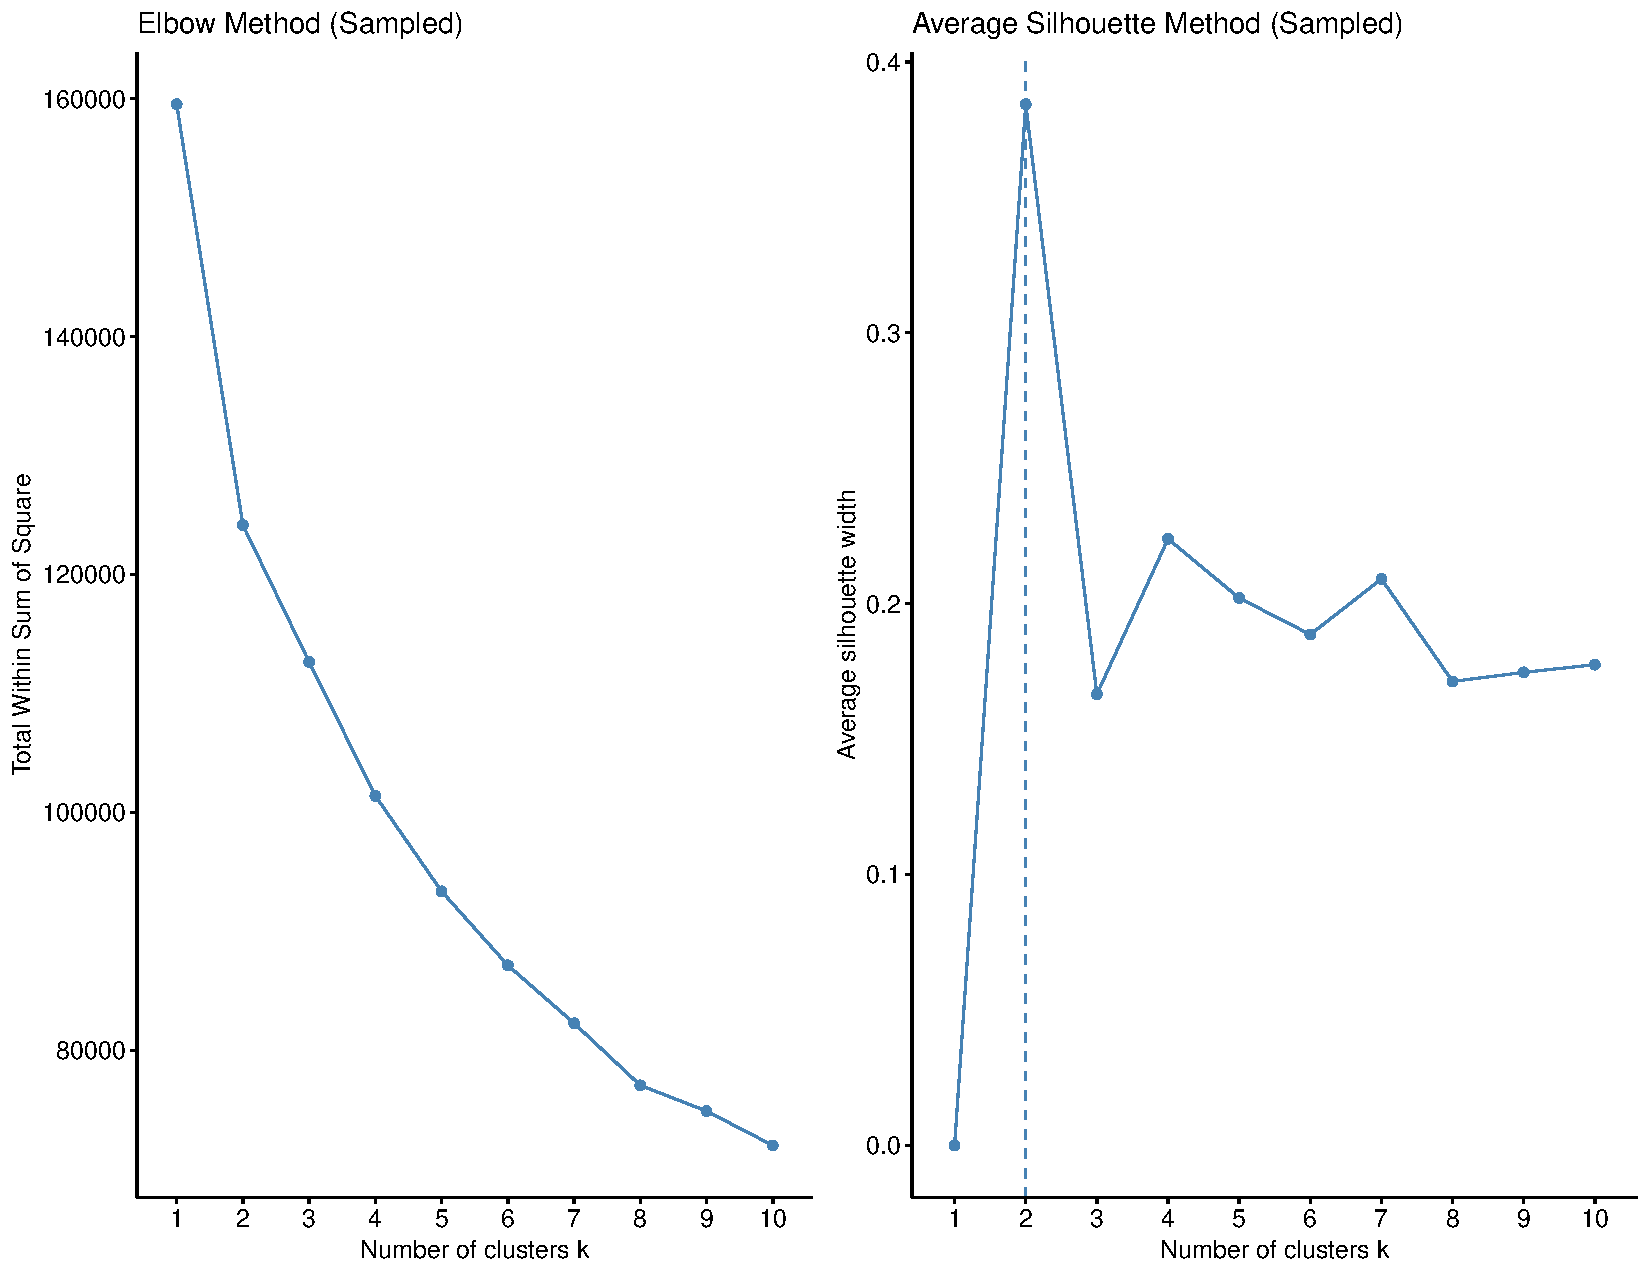
\includegraphics[scale=0.3]{k-means_diagnostic_plots.pdf}}
	\caption{K-Means Diagnostic Plots}
	\label{k-means_diagnostic_plots}
\end{figure} 

The Elbow plot shows a primary inflection point at $k=2$, representing the first major point of decrease before the reduction in Total Within Sum of Square (WSS) stabilizes.\\
\indent Concurrently, the Average Silhouette Method exhibits a clear peak at $k=2$ with a width of approximately $0.38$, indicating optimal cluster separation and cohesion. Consequently, $k=2$ was selected for the final model.

To evaluate the clustering results, the data was projected onto the first two principal components ($PC_1$ and $PC_2$), as they show greatest variance (Figure \ref{PCA_Combined_Scree_Plot}).\\
\indent Figure \ref{k-means_pca_PC1_PC2_k}, provides a representation of the spatial density and a visible boundary between the two identified clusters.

\begin{figure}[htbp]
	\centerline{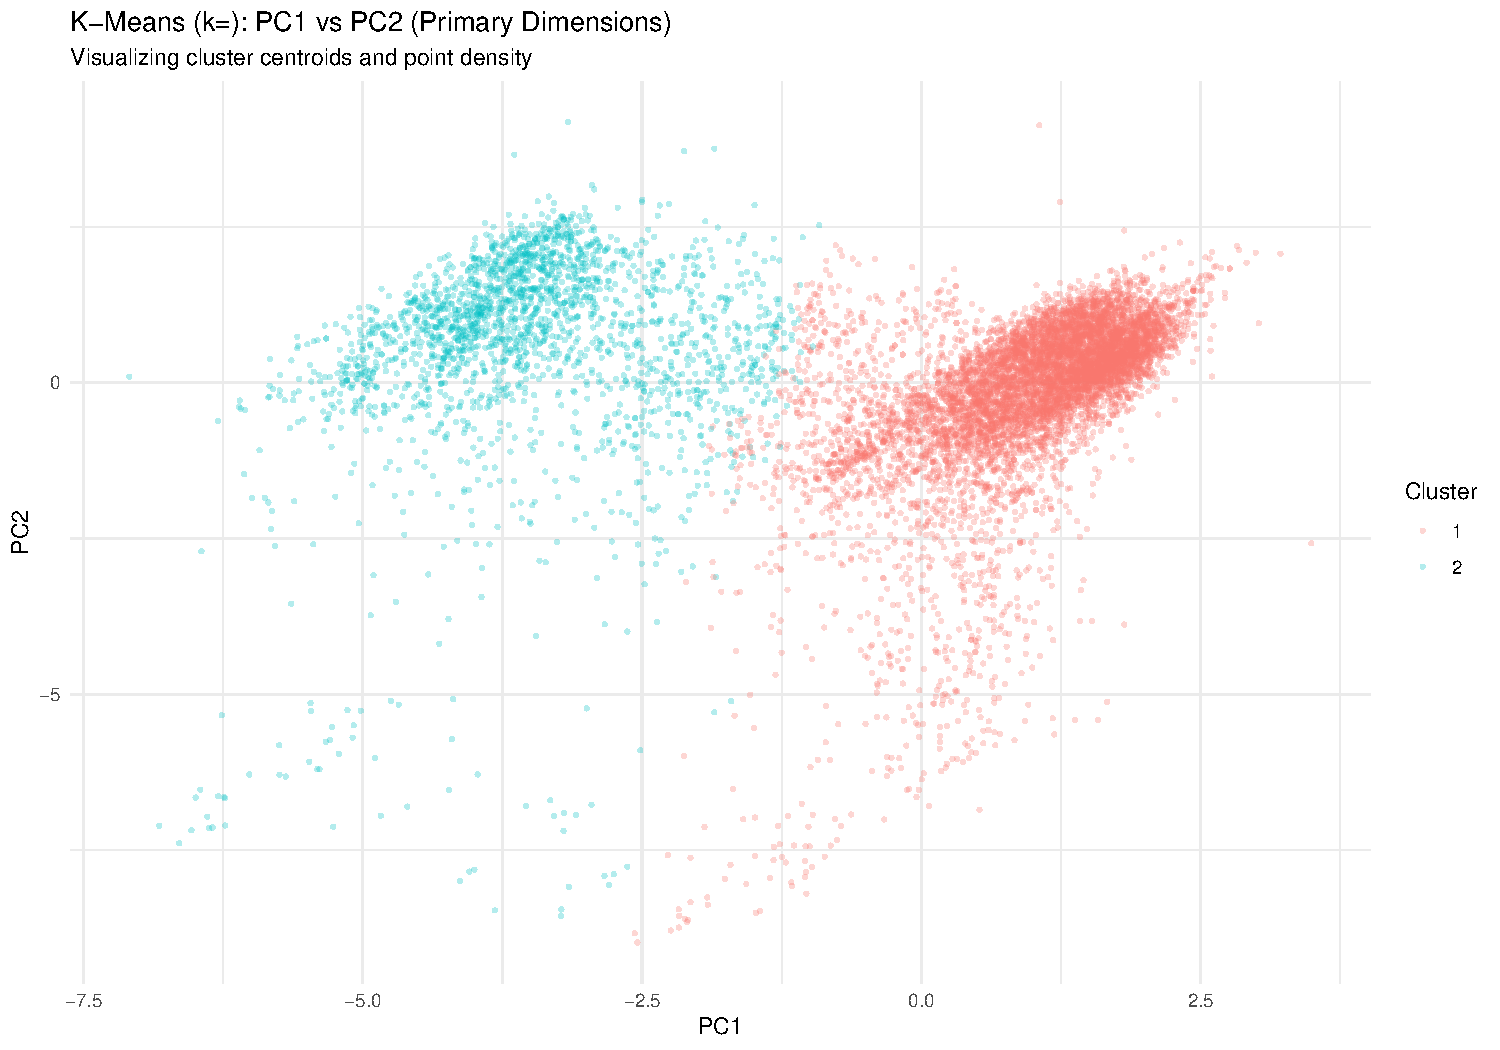
\includegraphics[scale=0.35]{k-means_pca_PC1_PC2_k.pdf}}
	\caption{K-Means $PC_1$ vs. $PC_2$}
	\label{k-means_pca_PC1_PC2_k}
\end{figure} 

\vspace{2mm}

\subsection{\textbf{Gaussian Mixture Model (GMM)}}

The optimal number of components for the \textbf{GMM} was determined using the Bayesian Information Criterion (BIC) \cite{ISLR2}.

\begin{figure}[htbp]
	\centerline{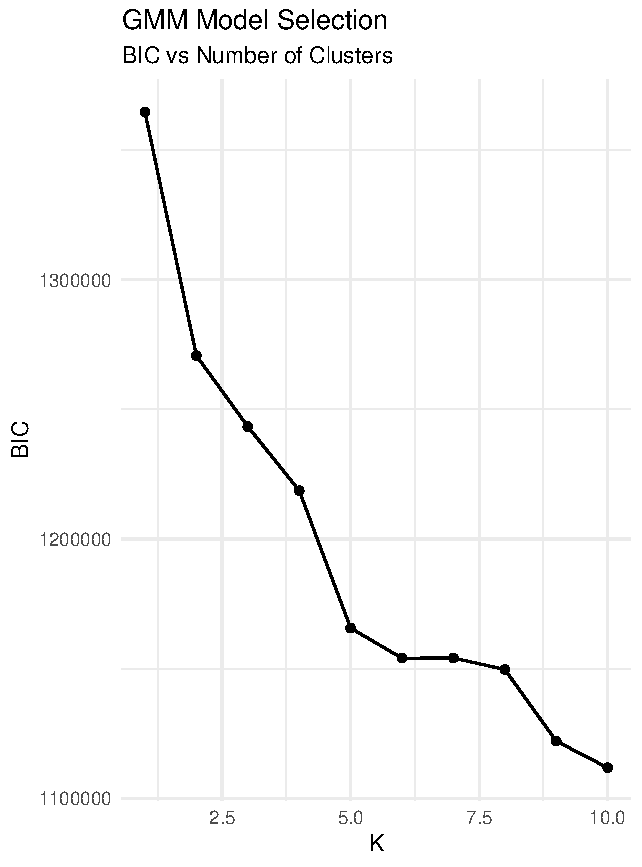
\includegraphics[scale=0.50]{gmm_bic_selection_plot.pdf}}
	\caption{BIC vs. K plot}
	\label{gmm_bic_selection_plot}
\end{figure} 

The BIC vs. K plot (Figure \ref{gmm_bic_selection_plot}) indicates a distinct elbow at $K=5$, where the criterion value begins to plateau, suggesting an optimal balance between model complexity and likelihood.

Based on this diagnostic, a five-component model was implemented.

The cluster assignments are visualized through a projection onto $PC_1$  and $PC_2$ , shown in Figure \ref{gmm_pca_PC1_PC2}. The plot shows how \text{GMM} probabilistic framework partitions the data along the dimensions of maximum variance. 

\begin{figure}[htbp]
	\centerline{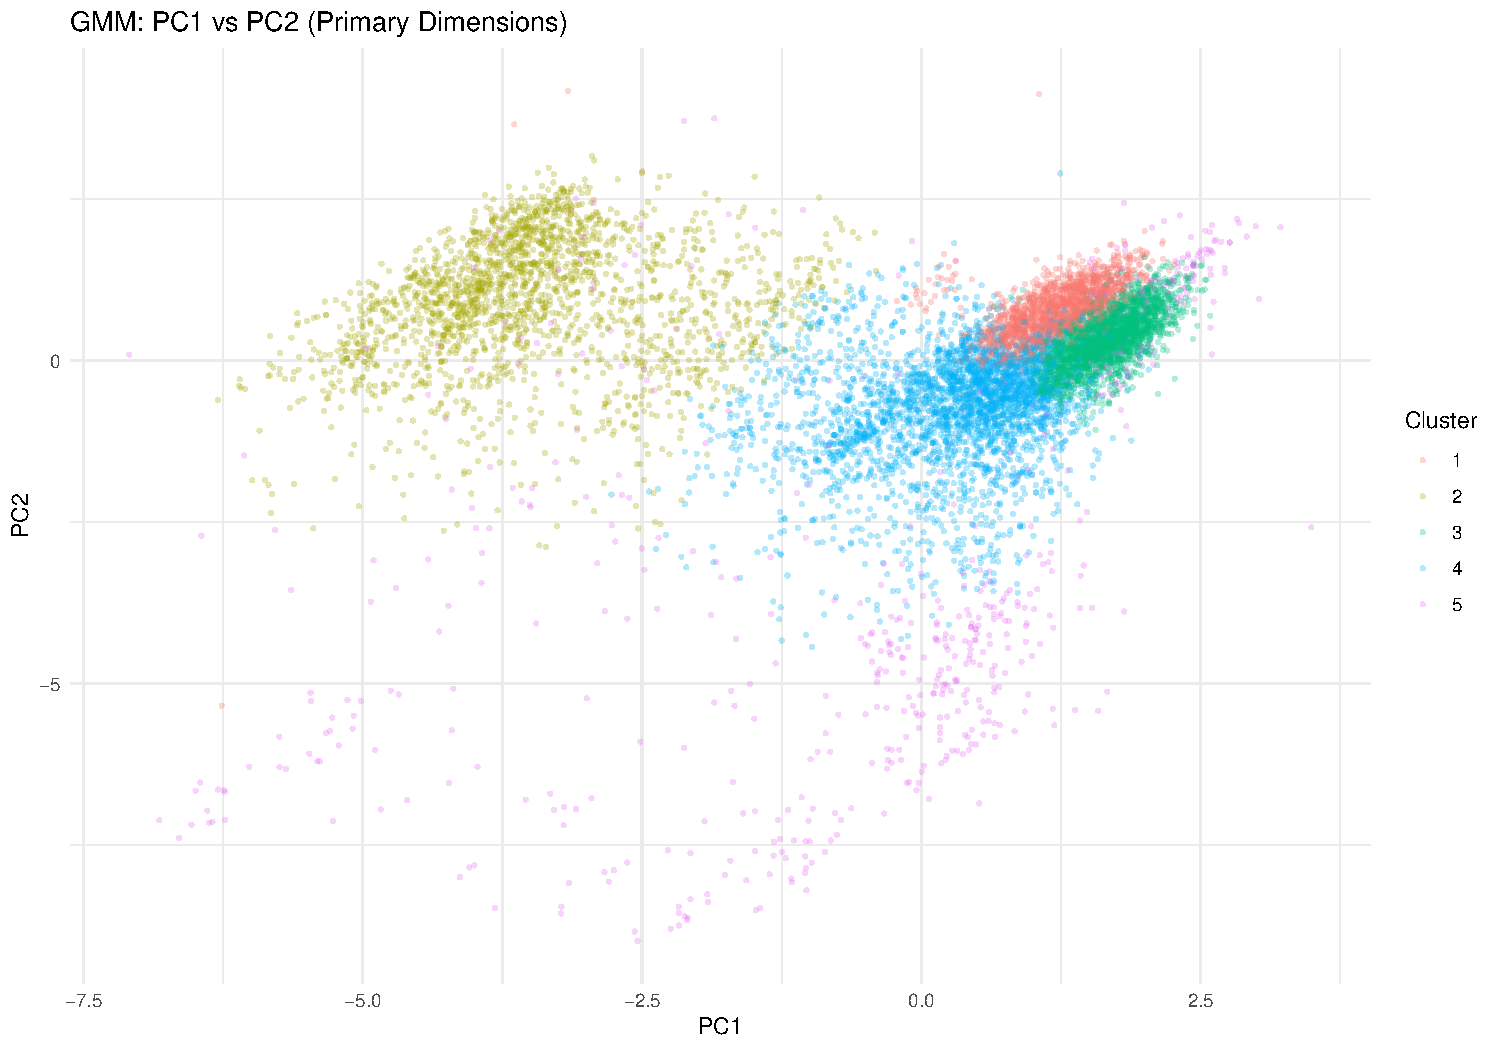
\includegraphics[scale=0.35]{gmm_pca_PC1_PC2.pdf}}
	\caption{GMM $PC_1$ vs. $PC_2$}
	\label{gmm_pca_PC1_PC2}
\end{figure} 

While three clusters overlap centrally, this suggests the model identified enough statistical distinctness in the underlying density to justify separate Gaussian components.

\vspace{2mm}

\subsection{\textbf{Spectral Clustering}}

The optimal number of clusters was determined using the Eigengap Heuristic (Figure \ref{spectral_eigengap_plot}), which examines the differences between consecutive eigenvalues of the Laplacian matrix.
\begin{figure}[htbp]
	\centerline{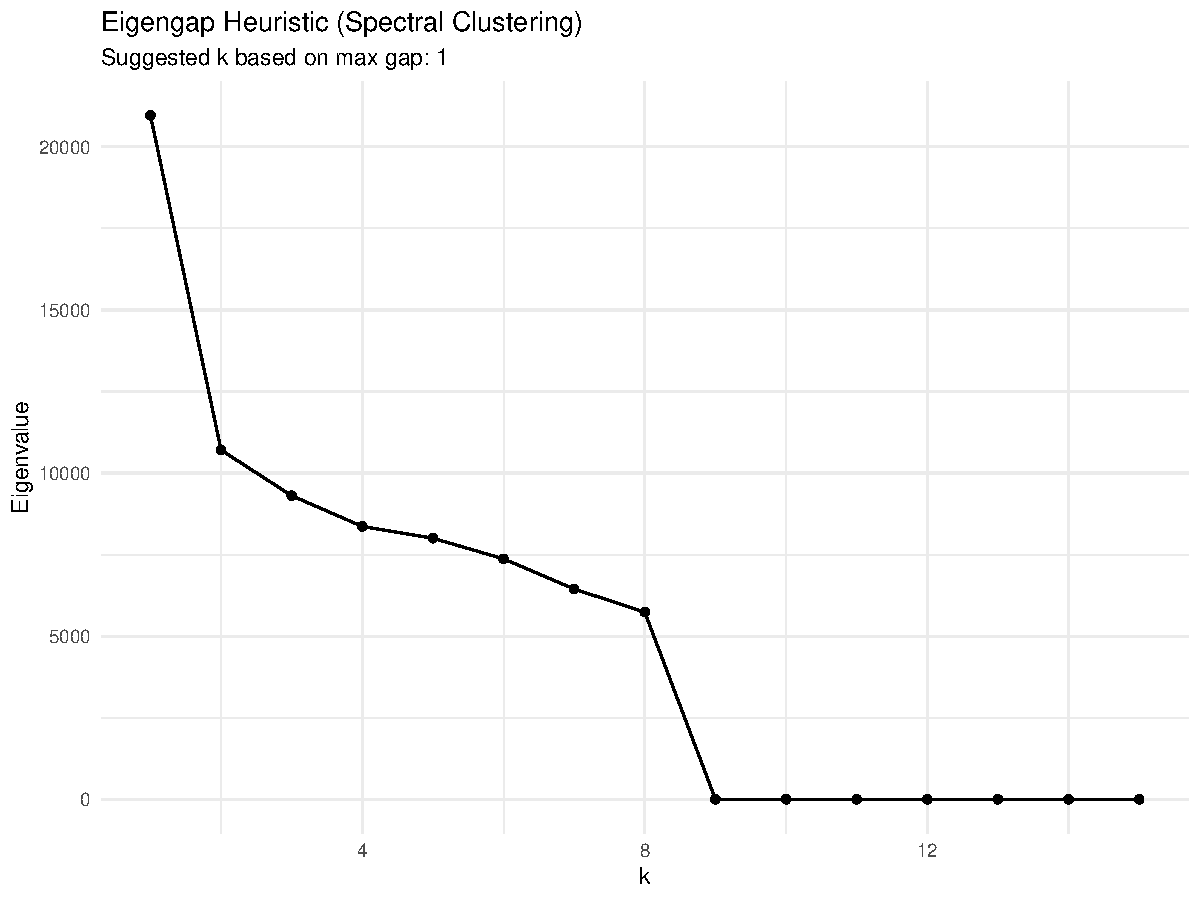
\includegraphics[scale=0.45]{spectral_eigengap_plot.pdf}}
	\caption{Eigengap Heuristic}
	\label{spectral_eigengap_plot}
\end{figure} 
While the largest gap is observed at $k=1$, a secondary prominent eigengap occurs at $k=8$, followed by a descent of eigenvalues toward zero. Consequently, $k=8$ was chosen to partition the data.

The resulting eight clusters are visualized using a \textbf{PCA} projection of $PC_1$ vs. $PC_2$ (Figure \ref{spectral_pca_PC1_PC2}).
This visualization is essential for interpreting how \textbf{Spectral Clustering} aligns with the primary dimensions of variance. Notably, where the \textbf{GMM} (Figure \ref{gmm_pca_PC1_PC2}) identified three overlapping clusters in the central population, the \textbf{Spectral Clustering} model concentrates the majority of its eight clusters within that middle structure. Only two clusters are positioned on the periphery, appearing distinct enough to be isolated from the dense central concentration.

\begin{figure}[htbp]
	\centerline{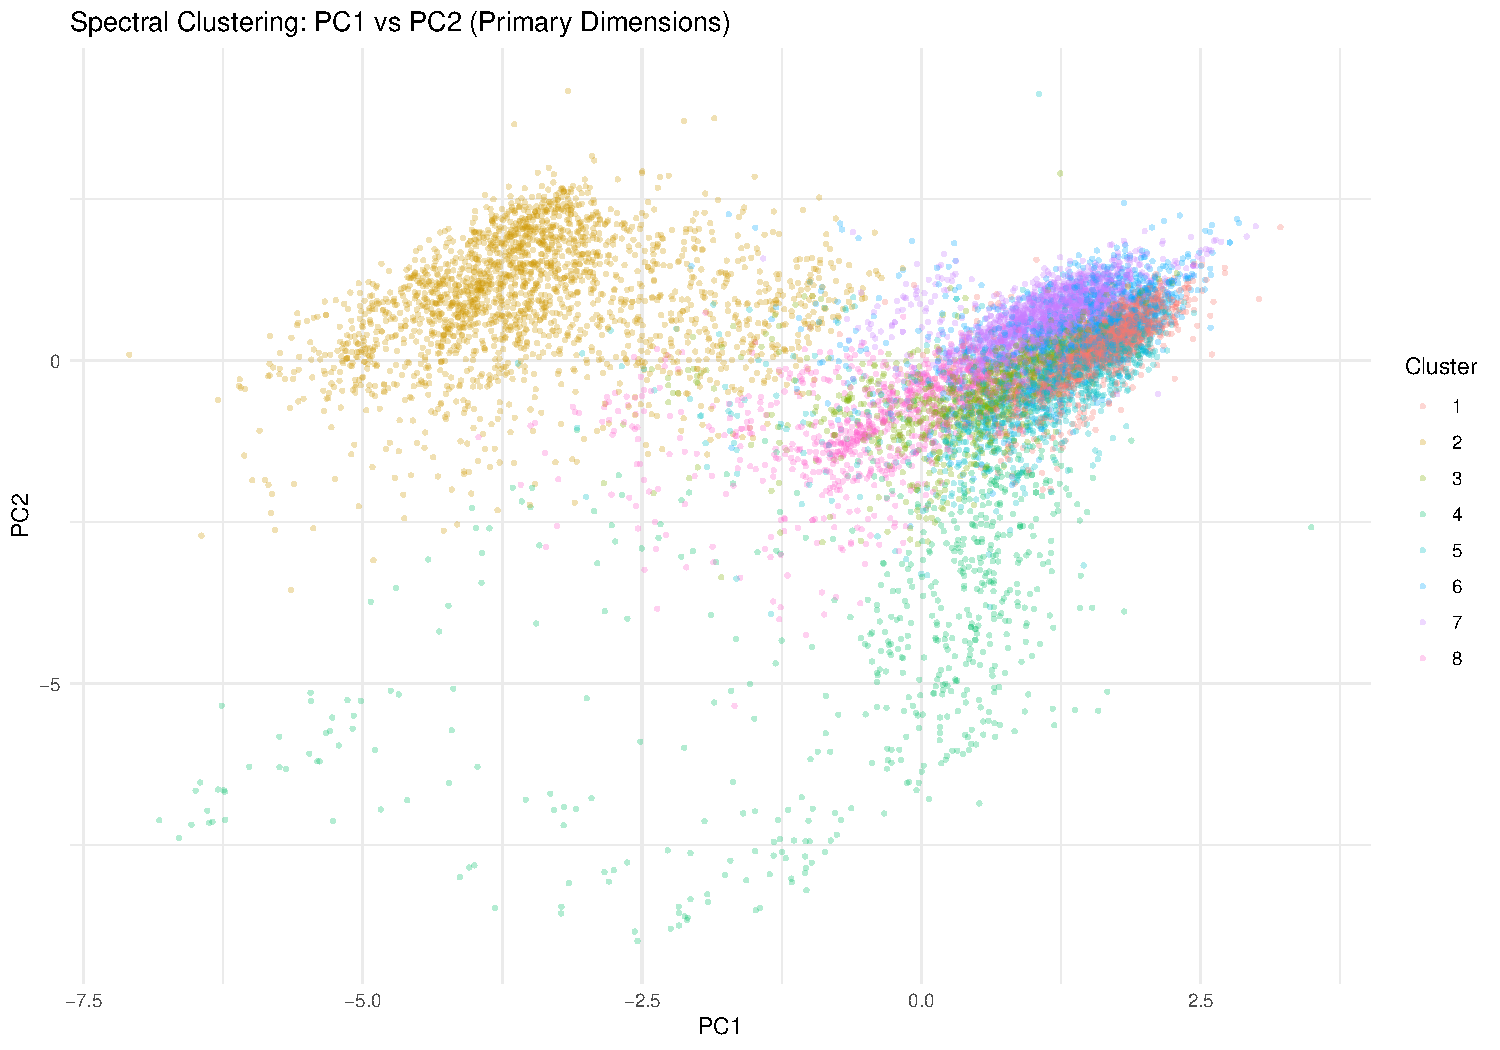
\includegraphics[scale=0.35]{spectral_pca_PC1_PC2.pdf}}
	\caption{Spectral $PC_1$ vs. $PC_2$}
	\label{spectral_pca_PC1_PC2}
\end{figure} 


\subsection{\textbf{Overall}}
The models reveal diverging interpretations of the dataset's structure. While \textbf{K-means} and \textbf{GMM} favor broader partitions ($k=2, 5$), \textbf{Spectral Clustering} identifies a higher granularity ($k=8$) within the central population.\\
\indent These varying results regarding spatial density and cluster stability provide the empirical basis for the comparative analysis to follow.


\section{\textbf{Discussion}}

\subsection{\textbf{Performance Metrics Comparison}}

\begin{table}[ht]
	\centering
	\caption{Clustering Performance Metrics Comparison}
	\label{tab:performance_metrics}
	\resizebox{\columnwidth}{!}{%
		\begin{tabular}{l|ccc}
			\hline
			\textbf{Model} & \textbf{Silhouette} & \textbf{Davies-Bouldin} & \textbf{Calinski-Harabasz} \\ \hline
			K-Means ($k=2$)  & 0.3340 & 1.6410 & 2849.2485 \\
			GMM ($k=5$)      & 0.1369 & 2.2598 & 1393.8054 \\
			Spectral ($k=8$) & 0.1884 & 1.5871 & 1428.9544 \\ \hline
		\end{tabular}
	}
\end{table}

\begin{itemize}
	\item \textbf{K-Means ($k=2$):} Demonstrates the highest Silhouette Score ($0.3340$) and Calinski-Harabasz Index ($2849.2485$), indicating that the macro-level split provides the most distinct cluster separation.
	\item \textbf{GMM ($k=5$):} Shows the highest Davies-Bouldin Index ($2.2598$), which is consistent with its probabilistic nature where cluster boundaries typically overlap more than in distance-based methods.
	\item \textbf{Spectral Clustering ($k=8$):} Provides the best (lowest) Davies-Bouldin Index ($1.5871$), suggesting that its granular clusters are highly compact and well-defined compared to the other models.
\end{itemize}

\indent The convergence of these metrics provides a case for valid interpretability. The high global scores of \textbf{K-Means} confirm a strong fundamental structure in the data, while the low Davies-Bouldin index for the \textbf{Spectral Clustering} model validates that even at a high granularity ($k=8$), the clusters remain compact and distinct.\\
\indent Additionally, the \textbf{GMM} metrics confirm that the density-based groupings are statistically grounded, successfully capturing the probabilistic overlaps and environmental nuances inherent in the dataset.\\
\indent Together, these results provide a robust statistical foundation, ensuring that the subsequent profiles are not artifacts of noise but represent meaningful, reproducible patterns within the dataset.

\subsection{\textbf{Comparative Analysis of Clustering Profiles}}

\begin{table}[ht]
	\centering
	\caption{Comparative Profile Centroids across Clustering Models}
	\label{tab:combined_clusters}
	
	% --- K-Means ---
	\centering K-Means Clustering Profiles
	\smallskip
	\resizebox{\columnwidth}{!}{
		\begin{tabular}{l|c|cc|ccc|c}
			\hline
			\textbf{Cluster} & \textbf{Severity} & \textbf{Temperature} & \textbf{Humidity} & \textbf{Crossing} & \textbf{Junction} & \textbf{Signal} & \textbf{Hour} \\ \hline
			Cluster 1 & -0.017 & 0.193 & -0.194 & 0.021 & -0.024 & 0.006 & 0.021 \\
			Cluster 2 & 0.062 & -0.695 & 0.697 & -0.076 & 0.087 & -0.021 & -0.075 \\ \hline
		\end{tabular}
	}
	
	\medskip % Vertical space between tables
	
	% --- GMM ---
	\centering GMM Clustering Profiles
	\smallskip
	\resizebox{\columnwidth}{!}{
		\begin{tabular}{l|c|cc|ccc|c}
			\hline
			\textbf{Cluster} & \textbf{Severity} & \textbf{Temperature} & \textbf{Visibility} & \textbf{Crossing} & \textbf{Junction} & \textbf{Signal} & \textbf{Hour} \\ \hline
			Cluster 1 & -0.320 & 0.240 & 0.328 & -0.007 & -0.137 & -0.170 & 0.352 \\
			Cluster 2 & 0.023 & -0.651 & 0.144 & -0.075 & 0.078 & -0.037 & -0.033 \\
			Cluster 3 & 0.060 & 0.801 & 0.329 & 0.125 & -0.000 & 0.071 & 0.354 \\
			Cluster 4 & 0.046 & -0.276 & -0.058 & -0.059 & 0.013 & 0.031 & -0.436 \\
			Cluster 5 & 0.267 & -0.391 & -2.551 & 0.055 & 0.038 & 0.111 & -0.012 \\ \hline
		\end{tabular}
	}
	
	\medskip
	
	% --- Spectral ---
	\centering Spectral Clustering Profiles
	\smallskip
	\resizebox{\columnwidth}{!}{
		\begin{tabular}{l|c|cc|ccc|c}
			\hline
			\textbf{Cluster} & \textbf{Severity} & \textbf{Temperature} & \textbf{Visibility} & \textbf{Crossing} & \textbf{Junction} & \textbf{Signal} & \textbf{Hour} \\ \hline
			Cluster 1 & 0.161 & 0.858 & 0.288 & -0.349 & 0.188 & -0.396 & 0.395 \\
			Cluster 2 & 0.047 & -0.633 & 0.144 & -0.079 & 0.089 & -0.043 & 0.007 \\
			Cluster 3 & -0.100 & -0.608 & 0.094 & -0.168 & 0.024 & -0.137 & -0.456 \\
			Cluster 4 & 0.135 & -0.383 & -3.080 & -0.163 & 0.056 & -0.088 & -0.252 \\
			Cluster 5 & 1.041 & 0.115 & 0.089 & -0.194 & 0.343 & 0.214 & -0.169 \\
			Cluster 6 & -0.543 & 0.471 & 0.246 & 1.183 & -0.525 & 0.977 & 0.159 \\
			Cluster 7 & -0.229 & 0.123 & 0.309 & -0.233 & -0.043 & -0.361 & 0.316 \\
			Cluster 8 & -0.206 & -0.303 & 0.026 & -0.100 & -0.074 & -0.048 & -0.749 \\ \hline
		\end{tabular}
	}
\end{table}

To understand the underlying patterns of the dataset, we compare the centroids of the unsupervised models.\\
\indent It is important to note that all values presented in Tables \ref{tab:combined_clusters} are \textbf{normalized (Z-score standardized)}, where $0$ represents the mean, positive values indicate features above the average, while negative values represent features below the average.\\
\indent To ensure interpretability, we mapped the Principal Components back to the original features using the rotation matrices saved during preprocessing. This allows for the analysis of clusters in terms of physical variables rather than abstract components.

\subsubsection*{\textbf{Discussion of Comparative Flow}}
To characterize the ``Perfect Storm" for traffic incidents in Florida, we examine the evolution of cluster signatures across three models.\\
\indent The transition from global to local patterns reveals how temporal, environmental, and situational factors converge to create high-risk signatures.

\begin{itemize}
	\item \textbf{K-Means (The Atmospheric Baseline):} 
	Establishes the macro-level environmental split. \textbf{Cluster 1} represents the ``Fair Weather" baseline (high temperature, low humidity), while \textbf{Cluster 2} isolates the ``Adverse Weather" state ($0.697$ humidity). This confirms that Florida's dataset is fundamentally divided by climate, though the minimal severity delta between these clusters suggests that weather alone is a precursor, not a singular cause, of high-risk events.
	
	\item \textbf{GMM (The Visibility Trigger):} 
	Refines the risk profile by isolating density-based outliers. \textbf{Cluster 5} identifies a critical ``Environmental Signature" where extreme low visibility ($-2.551$) directly correlates with a spike in Severity ($0.267$). This suggests that the "Perfect Storm" is not merely a "rain event" but specifically a \textit{visibility-deprivation event}, often occurring in the early morning or late evening.
	
	\item \textbf{Spectral Clustering (The Infrastructure Catalyst):} 
	Provides a granular view of the physical road environment. \textbf{Cluster 6} (The ``Protected Urban" signature) reveals that despite high infrastructure complexity (Signals $0.977$), severity is significantly lower ($-0.543$). Conversely, \textbf{Cluster 5} (The ``Vulnerable Junction" signature) identifies the highest severity in the study ($1.041$), occurring at junctions ($0.343$) that lack the mitigating presence of traffic signals or crossings.
\end{itemize}

\vspace{8mm}

\subsubsection*{\textbf{Synthesizing the 'Perfect Storm' Signature}}

The convergence of these models allows us to define the ``Perfect Storm" not as a single variable, but as a hierarchical intersection.\\
\indent While \textbf{K-Means} identifies the humid atmospheric backdrop and \textbf{GMM} isolates the visibility trigger, \textbf{Spectral Clustering} pinpoints the structural failure. 

Ultimately, the highest probability of a high-severity incident—the ``Perfect Storm"—is characterized by the \textbf{simultaneous occurrence of extreme visibility impairment ($Z < -2.5$) and the absence of traffic control measures at complex junctions.}\\
\indent This multi-model approach confirms that infrastructure is the decisive moderator: it determines whether a hazardous environment remains a signature or escalates into a high-risk event.

\vspace{8mm}

\section{\textbf{Conclusion}}

The ``Perfect Storm'' for traffic incidents in Florida is not a single environmental event, but a lethal convergence of atmospheric instability and infrastructure vulnerability.\\
\indent This study demonstrates that while adverse weather provides a high-risk backdrop, the transition from a hazardous environment to a high-severity crash is dictated by specific situational triggers.

\subsubsection*{\textbf{The ``Perfect Storm'' Signature Profile}}
The analysis explicitly identifies the highest-risk environmental signature as the intersection of:
\begin{itemize}
	\item \textbf{Extreme Visibility Impairment}: A critical deprivation event, typically occurring during off-peak hours.
	\item \textbf{Structural Failure}: The presence of complex road \textbf{junctions} lacking the mitigating protection of \textbf{traffic signals or crossings}.
\end{itemize}

By moving beyond univariate analysis, this study confirms that infrastructure acts as the decisive moderator of environmental danger.\\
\indent The ``Perfect Storm" is realized when these spatial gaps meet temporal instability, creating a specific, multi-dimensional window where crash probability is maximized.

\begin{thebibliography}{9}
	
% --- Dataset Requeried ---
	
\bibitem{moosavi2019countrywide}
Moosavi, S., Samavatian, M. H., Parthasarathy, S., \& Ramnath, R. (2019). 
\newblock A Countrywide Traffic Accident Dataset. 
\newblock \textit{arXiv preprint arXiv:1906.05409}.

\bibitem{moosavi2019accident}
Moosavi, S., Samavatian, M. H., Parthasarathy, S., Teodorescu, R., \& Ramnath, R. (2019). 
\newblock Accident Risk Prediction based on Heterogeneous Sparse Data: New Dataset and Insights. 
\newblock In \textit{Proceedings of the 27th ACM SIGSPATIAL International Conference on Advances in Geographic Information Systems} (pp. 33--42). ACM.

% --- General ---

\bibitem{ISLR2} 
James, G., Witten, D., Hastie, T., and Tibshirani, R. (2021). 
\textit{An Introduction to Statistical Learning: with Applications in R} (2nd ed.). 
Springer Texts in Statistics. New York: Springer.

% --- Dimensionality Reduction ---
\bibitem{Pearson1901} 
Pearson, K. (1901). 
\textit{On lines and planes of closest fit to systems of points in space}. 
Philosophical Magazine, 2(11), 559–572.

\bibitem{McInnes2018} 
McInnes, L., Healy, J., and Melville, J. (2018). 
\textit{UMAP: Uniform Manifold Approximation and Projection for Dimension Reduction}. 
arXiv preprint arXiv:1802.03426.

% --- Clustering Algorithms ---
\bibitem{MacQueen1967} 
MacQueen, J. (1967). 
\textit{Some methods for classification and analysis of multivariate observations}. 
Proceedings of the Fifth Berkeley Symposium on Mathematical Statistics and Probability, 1, 281–297.

\bibitem{Dempster1977} 
Dempster, A. P., Laird, N. M., and Rubin, D. B. (1977). 
\textit{Maximum Likelihood from Incomplete Data via the EM Algorithm}. 
Journal of the Royal Statistical Society: Series B (Methodological), 39(1), 1–22.

\bibitem{Ng2001} 
Ng, A. Y., Jordan, M. I., and Weiss, Y. (2001). 
\textit{On Spectral Clustering: Analysis and an algorithm}. 
Advances in Neural Information Processing Systems (NIPS), 14, 849–856.

% --- Evaluation Indices ---
\bibitem{Rousseeuw1987} 
Rousseeuw, P. J. (1987). 
\textit{Silhouettes: A graphical aid to the interpretation and validation of cluster analysis}. 
Journal of Computational and Applied Mathematics, 20, 53–65.

\bibitem{Davies1979} 
Davies, D. L., and Bouldin, D. W. (1979). 
\textit{A Cluster Separation Measure}. 
IEEE Transactions on Pattern Analysis and Machine Intelligence, (2), 224–227.

\bibitem{Calinski1974} 
Caliński, T., and Harabasz, J. (1974). 
\textit{A dendrite method for cluster analysis}. 
Communications in Statistics-Theory and Methods, 3(1), 1–27.

\section*{\textbf{Appendix}}

\section*{Appendix A: Supplementary Materials and Software Usage}
\subsection*{Source Code Repository \label{app:code}}
The source code, data, and detailed implementation scripts for this project are available on GitHub (URL: \url{https://github.com/gaguillen4384-dev/Data-Science/tree/main/DataMining_2/Risk_Profiles_Car_Accidents_Analysis}).

\subsection*{Software Usage Acknowledgment}
\begin{enumerate}
	\item The text and documentation were edited and refined using \textbf{Google Gemini}.
	\item \textbf{R} (version 4.x.x) was used for model computation and graphics development.
	\item The following \textbf{R} libraries were essential to the computational workflow:
\begin{itemize}
	\item \textbf{data.table}: Utilized for high-performance data manipulation and memory-efficient aggregation of the 881,605-record dataset.
	\item \textbf{dplyr}: Applied for intuitive data piping and grammatical transformations of situational and environmental variables.
	\item \textbf{lubridate}: Used for the precise parsing and extraction of temporal features from crash timestamps.
	\item \textbf{jsonlite}: Employed for the robust ingestion and flattening of nested JSON-formatted traffic data.
	\item \textbf{tidyr}: Used to pivot and reshape the dataset into the tidy formats required for multivariate clustering.
	\item \textbf{ggplot2}: Used as the primary engine for creating all statistical graphics and density plots of crash distributions.
	\item \textbf{patchwork}: Applied to combine multiple plots into cohesive, multi-panel figures for comparative analysis.
	\item \textbf{scales}: Utilized for formatting axis labels, adjusting color gradients, and managing non-linear transformations in visualizations.
	\item \textbf{tidyverse}: Employed as a meta-package to maintain a consistent data science workflow and dependency ecosystem.
	\item \textbf{fastDummies}: Used for the rapid creation of dummy variables from categorical infrastructure features like signage and junction types.
	\item \textbf{corrplot}: Applied for the visual exploration of correlation matrices to detect multicollinearity before dimensionality reduction.
	\item \textbf{reshape2}: Used for melting data structures to facilitate heatmaps and correlation visualizations.
	\item \textbf{GGally}: Utilized for the development of generalized pairs plots and parallel coordinate plots to visualize cluster separation.
	\item \textbf{ClusterR}: Employed for the efficient implementation of the Gaussian Mixture Models (GMM) and K-Means algorithms.
	\item \textbf{cluster}: Used for basic clustering utilities and the computation of the Silhouette Profile.
	\item \textbf{factoextra}: Applied for the elegant visualization of PCA results and the determination of optimal cluster counts via "elbow" and "gap" methods.
	\item \textbf{clusterSim}: Used to calculate the Davies-Bouldin (DB) and Calinski-Harabasz (CH) validation indices.
	\item \textbf{gridExtra}: Utilized for the low-level arrangement of graphical objects and table grobs within analysis reports.
	\item \textbf{fpc}: Employed for flexible procedures for clustering, including the computation of cluster stability and validation statistics.
	\item \textbf{kernlab}: Used for the implementation of the kernel-based methods required for Spectral Clustering at vulnerable junctions.
	\item \textbf{uwot}: Applied for the implementation of the Uniform Manifold Approximation and Projection (UMAP) for non-linear dimensionality reduction.
\end{itemize}
\end{enumerate}

	
\end{thebibliography}

\vspace{12pt}

\end{document}
